%!TEX root = ../terrainbook.tex
% chktex-file 46

\setchapterpreamble[u]{\margintoc}
\graphicspath{{gdem/figs/}}


\chapter{Global digital elevation models}% or global terrains
\label{chap:gdem}

We define as ``global digital elevation models'' (or global terrains) the datasets that cover (most of) the Earth (gDEM below).%
\index{global DEM}
Those datasets require different acquisition methods from local datasets, since flying an airplane or performing local surveys at the scale of the Earth is not really feasible (or is it?).
The acquisition instruments used must be \emph{space-borne}, \ie\ mounted on a satellite for instance.
Notice that the orbit of some satellites makes them technically non-global, but that we still refer to their datasets as global since they have a wide coverage, just restricted to certain latitudes.

Global DEMs are useful in several applications, they can be used as is or a derived product from a DEM is used (\eg\ slope or roughness).
Besides their ubiquitous use in flood modelling (see Chapter~\ref{chap:runoff}).

especially for environmental studies such as geological studies, hydrological modelling, ecosystems dynamics.

a few examples are the detection geological structures, the analysis of tectonic evolution, flood modelling, and the understanding of volcanic processes.


gDEMS have several properties and characteristics that apply only to them, and we report in this chapter on the main ones.
% We first describe global acquisition techniques, then we discuss the properties (and errors and biases, etc.) that the datasets collected will have, 



%%%%%%%%%%%%%%%%%%%%
%
\section[Acquisition of global data]{Acquisition of global elevation data}

The acquisition of gDEMs requires the use of a sensor mounted on a satellite.

The first gDEM (SRTM v1) was constructed with InSAR and released in 2003. 

As an alternative to InSAR and images from satellite is lidar.



%%%
\subsection{InSAR}

See Section~\ref{sec:insar}.


%%%
\subsection{Photogrammetry from high-resolution satellite images}

See Section~\ref{sec:photogrammetry}.

%%%
\subsection{Space lidar (ICESat-2 + GEDI)}

Lidar was first used in space on the Apollo missions, and with further technological developments, it has been used extensively from the 1990s onwards.
For example, Mercury, Mars, near-Earth asteroids, and lately again the moon have been scanned using lidar.

%

Earth surface elevation lidar measurements have also been developed, often flown on the Space Shuttles.
ICESat was the first Earth-based lidar satellite, launched in 2003, with the primary goal of ice sheet monitoring.
It had an elevation accuracy of several cm and was operational for five years.

%

NASA launched in 2018 two missions measure the elevation of the Earth globally with lidar instruments: 

\begin{itemize}
  \item \textbf{ICESat-2}
  \marginnote{\url{https://icesat-2.gsfc.nasa.gov/}} 
  (Ice, Cloud, and Land Elevation Satellite-2) is in a low Earth and polar orbit to investigate ice sheets, it covers the Earth between \ang{-88} and \ang{88} latitude.
  Its instrument to measure altimetry is called \emph{Advanced Topographic Laser Altimeter System} (ATLAS). 
  Apart from terrain retrieval, ICESat-2 also measures the surface, such as canopy height, and has many other applications such as measuring bathymetry and estimating biomass.
  \item \textbf{GEDI}
  \marginnote{\url{https://gedi.umd.edu/}} 
  (Global Ecosystem Dynamics Investigation) is attached to the international space station (ISS) and its main goal is to investigate global ecosystems.
  It does not have global coverage since it collects measurements only between \ang{51.6} N and \ang{51.6} S.
  GEDI has been combined with TanDEM-X data to produce biomass estimates and with Landsat imagery to produce a global canopy height map.
\end{itemize}
\begin{figure}
  \centering
  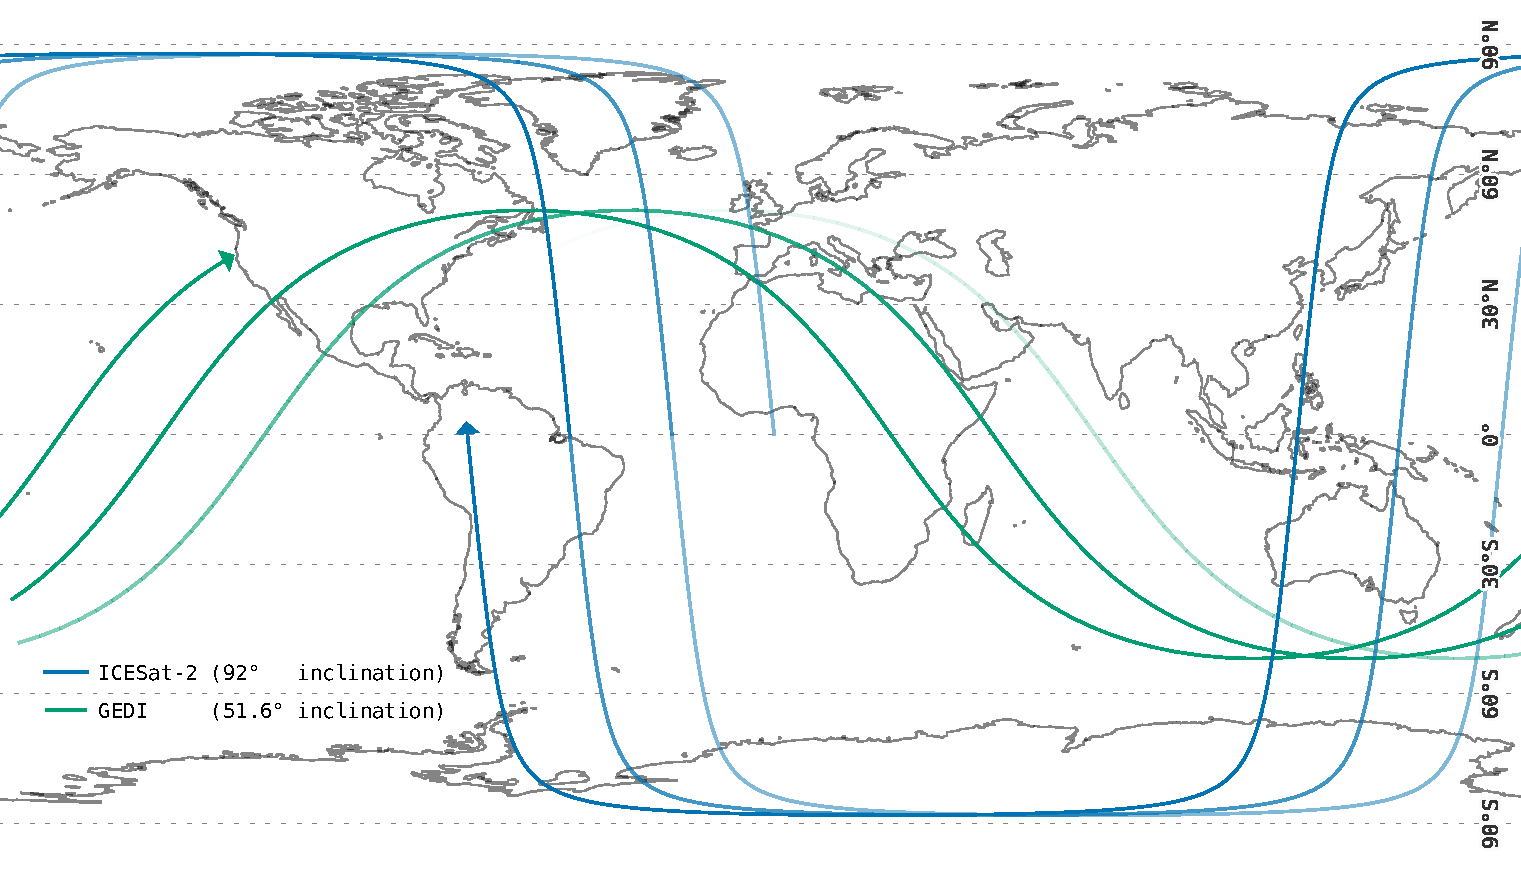
\includegraphics[width=\linewidth]{orbit}
  \caption{Three successive ground tracks for ICESat-2 and GEDI\@. Note the increased density of ground tracks at the latitude of inclination, as well as the lack of coverage beyond \ang{51.6}~latitude for GEDI.}%
\labfig{fig:orbit}
\end{figure}

%

The characteristics of both missions are summarised in Table~\ref{tab:lidarcomparison}
\begin{table*}
  \sisetup{detect-weight=true,detect-inline-weight=math}
  \caption{Key characteristics of GEDI and ICESat-2 missions in comparison with a typical airborne lidar mission.}
  \centering
  \begin{tabular}{llll}
    \toprule
                  & ICESat-2                             & GEDI                                   & airborne lidar\\
    \midrule
    \ type                 & discrete photon                      & full waveform                          & either           \\
    \ objective            & cryosphere monitoring                & Ecosystems                             & -                \\
    \ duration             & 2019-2022                            & 2019-2021                              & single flight(s) \\
    \ orbit inclination    & \ang{92}                             & \ang{51.6}                             & NA               \\
    \ laser pulse power    & \qty{175}{{\mu}J}/\qty{45}{{\mu}J}   & \qty{10000}{{\mu}J}/\qty{5000}{{\mu}J} & NA               \\
    \ elevation            & \qty{\pm480}{km}                     & \qty{\pm420}{km}                       & \qty{0.5}{km}    \\
    \ beam footprint       & \qty{17}{m}                          & \qty{23}{m}                            & \qty{0.05}{m}    \\
    \ along track spacing  & \qty{0.7}{m}                         & \qty{70}{m}                            & \qty{0.1}{m}     \\
    \ across track spacing & \qty{3}{km}/\qty{90}{m} between pair & \qty{0.6}{km}                          & \qty{0.1}{m}     \\
    \ swath width          & \qty{6.6}{km}                        & \qty{4.2}{km}                          & \qty{1}{km}      \\
    \ beam frequency       & \qty{512}{nm} (green)                & \qty{1064}{nm} (near-infrared)         & Either           \\
    \ \# beams             & 6 (in 3 pairs)                       & 8                                      & 1                \\
      \bottomrule
  \end{tabular}%
\label{tab:lidarcomparison}
\end{table*}

%

%%%
\paragraph{Strong and weak beams.}
Both missions have multiple laser beams and a division in beam energy, resulting in weak and strong beams (see Figure~\ref{fig:beams}).
\begin{figure}
  \centering
  \includegraphics[width=0.8\linewidth]{tracks}
  \caption{Filtered ICESat-2 and GEDI points from a single granule each at the 47th latitude, demonstrating the beam patterns.
  Note that ICESat-2 has a smaller beam footprint and a much higher pulse repetition, but a more uneven spatial coverage than GEDI\@.
  The gaps between data here will decrease by using multiple granules, but will never disappear completely.}%
\label{fig:beams}
\end{figure}
Weak beams (or coverage beams) are a way to improve coverage while still maintaining the mission requirement(s) for a specific power level with the strong beams.
Coverage is further increased for both missions by the ability to angle the instruments away from their reference ground tracks, preventing repetitions of the same ground track.
ICESat-2 lasers split into six beams, divided into three pairs, each pair \qty{90}{m} apart and the pairs \qty{3.3}{km} apart, for a total swath width of \qty{6.6}{km}.
Each pair contains a strong beam and a weak beam, with a power ratio of 4:1.
Along-track, it can measure each \qty{0.7}{m}, while its beam footprint is \qty{\pm17}{m}, so each measurement overlaps.
GEDI sensor has eight beams, each \qty{600}{m} apart, for a total swath width of \qty{4.2}{km}.
Of the eight beams, four are strong while the other four are weak beams, with a power ratio of 3:1.
GEDI measures a point every \qty{70}{m} along-track, with a beam footprint of \qty{23}{m}.
There are also notable differences between ICESat-2 and GEDI\@.
ICESat-2 has a high pulse repetition, the along track resolution is \qty{0.7}{m} for a footprint of \qty{17}{m}, each footprint thus overlaps other footprints significantly.
GEDI has no overlapping footprints, as its along track resolution is 100 times lower than ICESat-2.
Furthermore, whereas GEDI employs a full-waveform laser at a typical near-infrared wavelength of \qty{1064}{nm}, ICESat-2 employs a single-photon LiDAR at a bathymetric ``green'' wavelength of \qty{512}{nm}.
These differences stem from the different mission objectives: GEDI's full-waveform is excellent at deriving canopy structure, whereas ICESat-2's single-photon laser at \qty{512}{nm} is optimized for measuring ice elevation with an accuracy of centimetres, improving on the \qty{1064}{nm} laser used in the first ICESat mission.

%

%%%
\paragraph{Product levels.}
The data from the ICESat-2 and GEDI missions is made publicly available in several data products, categorised in 3 levels (Level 1, 2, and 3 data products), where a higher-level is derived from a lower-level product.
\begin{enumerate}
  \item \textbf{Level 1} products contains the raw telemetry;
  \item \textbf{Level 2} products contain directly usable geolocated data to which several corrections---such as accounting for atmospheric effects---are applied.
  \item \textbf{Level 3} data are aggregated versions of Level 2 products, which are smaller in filesize and easier to process.
  ICESat-2 differentiates between a Level 3A, which are aggregated Level 2 data products per \emph{granule}, and a Level 3B, which are gridded versions of the aggregated Level 3A data products.
  GEDI's Level 3 data product are gridded versions of Level 2 data products, like ICESat-2's Level 3B.
  GEDI also has Level 4 data products, which are model outputs---like carbon estimates---based on Level 2 data.
\end{enumerate}

%%%
\paragraph{Comparison to typical airbone lidar.}
These space borne lasers also differ considerably from airborne lasers, most notably so in their platform, resulting in significant differences in beam footprint and ground coverage.
The altitude increase results in a wider beam footprint, from \qty{\sim0.5}{m} (at \qty{500}{m}) for airborne platforms to \qty{\sim15}{m} for space platforms.
Although much wider, it is a small increase compared to the increase in altitude, going from \qty{0.5}{km} to \qty{480}{km}.
A comparison is given in Table~\ref{tab:lidarcomparison}.
Airborne LiDAR often focuses on maximizing coverage (\unit{points/m^2}) of smaller areas, whereas the coverage for space lasers is the ground track of the satellite.
While both ICESat-2 and GEDI employ instruments with multiple (split) laser beams, including the ability to point the laser away from the ground track, all to maximize coverage, this still results in very sparse and uneven coverage as shown in Figure~\ref{fig:beams}.



%%%%%%%%%%%%%%%%%%%%
%
\section[Specific characteristics]{Specific characteristics of gDEMs}

\begin{itemize}
  \item often near-global, depends on the orbits
  \item CRS, especially vertical datums
  \item resolution (often in degrees)
  \item DSM (more than DTM)
  \item size of datasets
  \item void filling: \url{https://en.wikipedia.org/wiki/Shuttle_Radar_Topography_Mission#Void-filled_SRTM_datasets}
  \item errors
  \item integration with sea-level datasets
  \item accuracy affected by slope (most image-based products)
\end{itemize}


%%%%%%%%%%%%%%%%%%%%
%
\section[Most common products]{Most common products available}

We list only the ones available as open-access?
For instance AW3D is also available as 5m-grid, but €€€.

Maybe we should make our own table with paid products too? Like that table: https://github.com/DahnJ/Awesome-DEM#summary
I find it interesting to know that some products are not free, and way better

% TODO: remake the inheritance fig
\begin{figure}
  \centering
  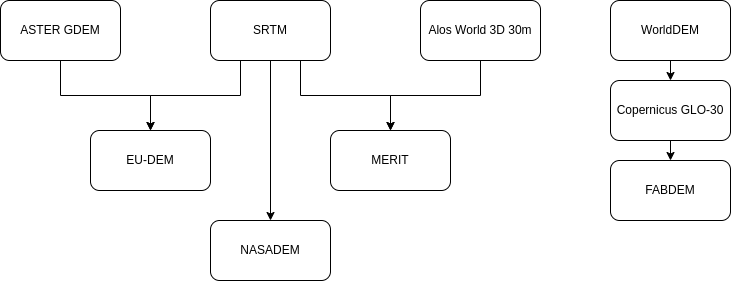
\includegraphics[width=\linewidth]{gdem_inheritance}
  \caption{(Figure from \url{https://github.com/DahnJ/Awesome-DEM})}%
\labfig{fig:gdem_inheritance}
\end{figure}


% TODO: put that image somehow: https://twitter.com/3vetion/status/1538934235679141888

\begin{itemize}
  \item ASTER
  \item AW3D30
  \item STRM
  \item CopernicusDEM
  \item MERIT
  \item FABDEM
  \item ICESat-2 (the gridded version?)
  \item GEDI (the gridded version?)
  \item global proprietary (\url{https://github.com/DahnJ/Awesome-DEM#worlddem-and-tandem-x})
\end{itemize}

A few words about fusion? [Okolie22] has very long review.


%%%%%%%%%%%%%%%%%%%%
%
\section{Conversion DSM to DTM}

Some examples of how done?

Or: correction bias for vegetations/trees and buildings (all man-made objects).

%%%%%%%%%%%%%%%%%%%%
%
\section{Notes \& comments}

\citet{Yang11} provide a detailed list of applications where gDEMs (SRTM, but when the paper was written (2011) SRTM was still the main product available globally) are necessary as input.
They 

Arguably the best place to download DEMs (gDEMS, local ones, lidar datasets, etc.) is OpenTopography (\url{https://opentopography.org}).




%%%%%%%%%%%%%%%%%%%%
%
\section{Exercises}

\begin{enumerate}
  \item What is what?
\end{enumerate}
